% Fakesection 序言之前

\RequirePackage[l2tabu, orthodox]{nag}
\RequirePackage{ifxetex}
\RequireXeTeX

\documentclass{article}

%颜色
\usepackage{xcolor}
\xdefinecolor{lightBlue}{rgb}{.22,.45,.7}
\xdefinecolor{darkGrey}{rgb}{.45,.45,.45}
\xdefinecolor{DeepSkyBlue}{RGB}{0, 104, 139}
\xdefinecolor{dkpurple}{rgb}{.455, .204, .506}

%长度
\usepackage{printlen}
\uselengthunit{mm}

%图形
\usepackage{media9}
\usepackage{pdfpages}
\usepackage{overpic}
\usepackage{graphicx}
\graphicspath{{./src/}}
\usepackage{wallpaper}
\usepackage{wrapfig}
\usepackage{pstricks}
\usepackage{tikz}
\usetikzlibrary{patterns}
\usetikzlibrary{arrows}
\usetikzlibrary{shapes}
\usetikzlibrary{chains}
\usetikzlibrary{mindmap}
\usetikzlibrary{graphs}
\usepackage{scsnowman}
\usepackage{tikzpeople}
\usepackage{tikzducks}
\usepackage{pifont}
\usepackage{marvosym}
%\usepackage{bbding}
\usepackage{stmaryrd}
\usepackage{ean13isbn}
\newcommand{\drawbarcode}[1]{\EANisbn[SC5a, ISBN = #1]}
\usepackage{qrcode}

%%进度条
\newcommand{\progressbar}[2][2cm]{%
	\textcolor{lightBlue}{\rule{#1 * \real{#2} / 100}{1.5ex}}%
	\textcolor{darkGrey!15}{\rule{#1 - #1 * \real{#2} / 100}{1.5ex}}
}

%表格
\usepackage{tabu}
\usepackage{longtable}
\usepackage{booktabs}
\usepackage{diagbox}
\usepackage{multicol}
\usepackage{multirow}
\usepackage{makecell}
\usepackage{fancybox}
\usepackage{colortbl}
\usepackage{tcolorbox}
\tcbuselibrary{skins}
\tcbuselibrary{breakable}
\tcbuselibrary{theorems}
\tcbuselibrary{listings}
\tcbuselibrary{xparse}
\usepackage{fvextra}
\usepackage{csvsimple}

%公式
\usepackage{amsmath}
\usepackage{amsthm}
\usepackage{amsfonts}
\usepackage{amssymb}
\usepackage{amsbsy}
\usepackage{amsopn}
\usepackage{amstext}
\usepackage{mathrsfs}
\usepackage{bm}
\usepackage{textcomp}
\usepackage{latexsym}
\usepackage{exscale}
\usepackage{relsize}
%\usepackage{xymtex}
\usepackage{physics}
\usepackage{siunitx}
\usepackage{hologo}
\usepackage{cases}

%正文
\usepackage{fancyhdr}
\usepackage{geometry}
\usepackage{lastpage}
\usepackage{indentfirst}
\usepackage{setspace}
\renewcommand\arraystretch{1.5}

%非正文
\usepackage{makeidx}
\makeindex
\usepackage{epigraph}
\usepackage{varwidth}

%参考文献
\usepackage{morewrites}
\renewcommand{\thefootnote}{\fnsymbol{footnote}}
\usepackage[resetlabels]{multibib}
\newcites{sec}{参考网站}

%%链接
\usepackage
[	colorlinks = true,
linkcolor = gray,
citecolor = gray,
backref=page
]{hyperref}
\usepackage{caption}
\usepackage{subcaption}
\DeclareCaptionLabelFormat{andtable}%
{#1#2~\&~\tablename\thetable}
%\renewcommand{\thetable}{\alph{table}}
%\renewcommand{\thefigure}{\Alph{table}}
%\renewcommand{\thesubtable}{\Roman{subtable}}
%\renewcommand{\thesubfigure}{\arabic{subfigure}}
%\captionsetup[figure]{labelfont=it,textfont={bf,it}}
%\captionsetup[subfigure]{labelfont=bf,textfont=normalfont,singlelinecheck=off,justification=raggedright}

%其它
\usepackage{atbegshi}
\newcommand{\handlethispage}{}
\AtBeginShipout{\handlethispage}
\usepackage{lipsum}

%枚举%与beamer冲突
\usepackage{enumitem}
\setlist[enumerate, 1]
{	fullwidth,
	label = \arabic*.,
	font = \textup,
	itemindent=2em
}

\csname
endofdump
\endcsname

\bibliographystyle{IEEEtran}
\bibliographystylesec{IEEEtran}
%\usepackage[notref,notcite]{showkeys}

%文字
\usepackage{csquotes}
\usepackage{ctex}
%\xeCJKsetup{
%	CJKecglue = {\hskip .10em plus .05em minus .05em},
%	CheckSingle = true
%}
%\setCJKmainfont[
%	BoldFont = {Noto Serif CJK SC Bold},
%	ItalicFont = {AR PL UKai HK}
%]{Noto Serif CJK SC ExtraLight}
%\setCJKsansfont[
%	BoldFont = {Noto Sans S Chinese Medium},
%	ItalicFont = {Noto Sans S Chinese DemiLight}
%]{SimSun}
%\setCJKmonofont[
%	BoldFont = {Adobe Heiti Std},
%	ItalicFont = {Adobe Kaiti Std}
%]{WenQuanYi Micro Hei Mono Light}
%\setCJKfamilyfont{zhkesong}{MF KeSong (Noncommercial)}
%\setCJKfamilyfont{zhhjsd}{MF TheGoldenEra (Noncommercial)}
%\setCJKfamilyfont{zhlangsong}{MF LangSong (Noncommercial)}
%\newcommand{\hjsd}{\CJKfamily{zhhjsd}}
%\newcommand{\KeSong}{\CJKfamily{zhkesong}}
%\newcommand{\langsong}{\CJKfamily{zhlangsong}}
%\newfontfamily\KeSongf[Mapping = tex-text]{MF KeSong (Noncommercial)}
%\newfontfamily\hjsdf[Mapping = tex-text]{MF TheGoldenEra (Noncommercial)}
%\newfontfamily\langsongf[Mapping = tex-text]{MF LangSong (Noncommercial)}
%\newfontfamily\SourceCodePro[Mapping = tex-text]{Source Code Pro}
%\newfontfamily\monaco{Monaco}
%\usepackage{microtype}

%%代码
\ifnum\shellescape=1
	\usepackage{minted}
	\tcbuselibrary{minted}% 用minted排版代码
\fi
%Java %与mcode冲突
% \usepackage{lstcustom}
%Matlab %与lstcustom冲突
%\usepackage[framed,numbered,autolinebreaks,useliterate]{mcode}
\usepackage{boxie}
\makeatletter
\xdefinecolor{tcbcol@back}{rgb}{0,0,0}
\makeatother
\renewcommand*\lstlistingname{代码}

%枚举%与beamer冲突
\usepackage{enumitem}
\setlist[enumerate, 1]
{	fullwidth,
	label = \arabic*.,
	font = \textup,
	itemindent=2em
}
\setlist[enumerate, 2]
{	fullwidth,
	label = \alph*.,
	font = \textup,
	itemindent=2em
}

\title{\textbf{基于图论的军事通信网络优化设计与抗毁性研究}}
\author{}
\date{}

%页眉页脚%与book冲突
\pagestyle{fancy}
\renewcommand{\headrulewidth}{0pt}
\lhead{}
\chead{}
\rhead{}
\lfoot{\small{\leftmark}}
\cfoot{\small{第\thepage 页~共~\pageref{LastPage}~页}}
%\rfoot{\small{\rightmark}}
\usepackage{titlesec}
%\titleformat{\chapter}{\centering\Huge\bfseries}{实验\chinese{chapter}~}{4mm}{}
\titleformat{\section}{\centering\LARGE\bfseries}{\S\ifthenelse{\value{section}=0}{}{\thesection}}{3mm}{}
%\titleformat{\subsection}{\Large}{\chinese{subsection}、}{2mm}{}
%\titleformat{\subsubsection}{\large}{\arabic{subsubsection}.}{1mm}{}
\renewcommand{\abstractname}{\Large 摘要}

\begin{document}

% Fakesection 承诺书

\newcommand{\NumberMilitaryMathModeling}{B028819084}
\newcommand{\NumberNJUSTMathModeling}{114}
\newcommand{\NumberProblem}{B}
\newcommand{\MemberOne}{吴振宇}
\newcommand{\MemberTwo}{张文奇}
\newcommand{\MemberThree}{谷鑫}
\newcommand{\MemberTeacher}{}
\newcommand{\MembersUniversity}{南京理工大学}
\newcommand{\MembersCollege}{电子工程与光电技术学院、机械工程学院}
\newcommand{\Year}{2019}
\newcommand{\Month}{5}
\newcommand{\Day}{4}

\newif\ifMilitaryMathModeling\MilitaryMathModelingfalse
\newif\ifNJUSTMathModeling\NJUSTMathModelingfalse
\newif\ifNoAppendix\NoAppendixfalse

\newcounter{NumberSessionMilitaryMathModeling}
\setcounter{NumberSessionMilitaryMathModeling}{\Year}
\addtocounter{NumberSessionMilitaryMathModeling}{-2016}
\ifnum\strcmp{\jobname}{\NumberMilitaryMathModeling}=0
	\MilitaryMathModelingtrue
\fi
\ifnum\strcmp{\jobname}{\NumberNJUSTMathModeling}=0
	\NJUSTMathModelingtrue
\fi
\ifnum\strcmp{\jobname}{NJUST}=0
	\NJUSTMathModelingtrue
	\NoAppendixtrue
\fi
\ifnum\strcmp{\jobname}{main}=0
	\MilitaryMathModelingtrue
	\NJUSTMathModelingtrue
\fi

% Fakesubsection 军事数学建模

\ifMilitaryMathModeling

	\thispagestyle{empty}
	\newgeometry{left=2.5cm,right=2.5cm,top=2cm,bottom=2cm}

	\begin{center}
		\zihao{3}

		\textbf{第\chinese{NumberSessionMilitaryMathModeling}届全国大学生军事数学建模竞赛学术道德与保密承诺书}
	\end{center}

	\vspace{1em}

	\begin{spacing}{2.0}
		\fangsong
		\zihao{4}

		我们仔细阅读了第\chinese{NumberSessionMilitaryMathModeling}届全国大学生军事数学建模竞赛的竞赛章程。

		我们完全清楚,在竞赛开始后参赛队员不能以任何方式(包括电话、电子邮件、网上咨询等)与队外的任何人(包括指导老师)研究、讨论与赛题有关的问题。

		我们完全清楚,必须遵守保密规定,不能在互联网等非保密环境和设备上拷贝、张贴、上传、讨论竞赛题目和答卷,不能向任何队外人员传送竞赛题目和答卷。我们提交的竞赛论文等成果涉密等级不超过秘密。

		我们知道,抄袭别人的成果是违反竞赛规则的,如果引用别人的成果或其他公开的资料(包括网上查到的资料),必须按照规定的参考文献的表述方式在正文引用处和参考文献中明确列出。

		我们郑重承诺,严格遵守竞赛规则,以保证竞赛的公正、公平性。如有违反竞赛规则的行为,我们将受到严肃处理。

		我们参赛的题号是(从A、B、C、D中选择一项):\NumberProblem

		我们的参赛队号为:\NumberMilitaryMathModeling

		所属单位(填写全称):\MembersUniversity

		参赛队员:1.\underline{\makebox[8\ccwd][c]{\MemberOne}}2.\underline{\makebox[8\ccwd][c]{\MemberTwo}}3.\underline{\makebox[8\ccwd][c]{\MemberThree}}

		指导老师:\underline{\makebox[20\ccwd][c]{\MemberTeacher}}
	\end{spacing}

	\begin{flushright}
		\fangsong
		\zihao{4}

		日期:\Year 年\Month 月\Day 日
	\end{flushright}

	\restoregeometry
	\setcounter{page}{1}

\fi

% Fakesubsection 南京理工大学数学建模

\ifNJUSTMathModeling

	\thispagestyle{empty}
	\newgeometry{left=2.5cm,right=2.5cm,top=3cm}

	\begin{center}
		\textbf{\zihao{4}\Year 南京理工大学大学生数学建模竞赛}

		\vspace{2em}

		\textbf{\zihao{3}承~诺~书}

		\vspace{1em}
	\end{center}

	{\zihao{-4}

		我们仔细阅读了中国大学生数学建模竞赛的竞赛规则.

		我们完全明白,在竞赛开始后参赛队员不能以任何方式(包括电话、电子邮件、网上咨询等)与队外的任何人(包括指导教师)研究、讨论与赛题有关的问题。

		我们知道,抄袭别人的成果是违反竞赛规则的, 如果引用别人的成果或其他公开的资料(包括网上查到的资料),必须按照规定的参考文献的表述方式在正文引用处和参考文献中明确列出。

		我们郑重承诺,严格遵守竞赛规则,以保证竞赛的公正、公平性。如有违反竞赛规则的行为,我们将受到严肃处理。

		我们授权全国大学生数学建模竞赛组委会,可将我们的论文以任何形式进行公开展示(包括进行网上公示,在书籍、期刊和其他媒体进行正式或非正式发表等)。

		我们参赛选择的题号是(从A/B中选择一项填写):\underline{\makebox[12\ccwd][c]{\NumberProblem}}

		我们的参赛报名号为(报名编号):\underline{\makebox[12\ccwd][c]{\NumberNJUSTMathModeling}}

		所属学院(请填写完整的全名):\underline{\makebox[20\ccwd][c]{\MembersCollege}}

		参赛队员(打印并签名):1.\underline{\makebox[12\ccwd][c]{\MemberOne}}

		\makebox[11.5\ccwd][c]{}2.\underline{\makebox[12\ccwd][c]{\MemberTwo}}

		\makebox[11.5\ccwd][c]{}3.\underline{\makebox[12\ccwd][c]{\MemberThree}}

		\begin{flushright}
			日期:\underline{\makebox[4\ccwd][c]{\Year}}年\underline{\makebox[4\ccwd][c]{\Month}}月\underline{\makebox[4\ccwd][c]{\Day}}日
		\end{flushright}

	}

	\hrulefill

	{\zihao{4}评阅编号(由组委会评阅前进行编号):}

	\restoregeometry
	\setcounter{page}{1}

\fi

% Fakesection 摘要

\maketitle

\begin{abstract}
	\zihao{5}

	党的十九大报告指出,加快军事智能化发展,提高基于网络信息体系的联合作战能力。在这一背景下,建设成本更低、抗毁性越高的军事通信网,成为保证战场信息畅通的关键。我们将通信问题抽象为图论问题,使用最小生成树Prim算法、最大流算法、重要节点强制摧毁算法等方法构建数学模型,提出了军事通信网络的优化方案。

	针对问题一,我们建立了 \textbf{最短链路设计模型} 。首先,我们利用城市经纬度计算城市间的距离;随后,利用最小生成树Prim算法构建通信线路总长度最短的网络连接方案。

	针对问题二,我们建立了 \textbf{针对独立割点城市的战备节点配置模型} 。首先,我们通过分类讨论确定战备节点最佳数量为3个;随后,我们以战备节点到摧毁点的距离大于安全距离为约束条件,从而确保安全性,又以战备节点距离相连城市的距离和最短为目标函数,从而确保经济性,求得战备节点的最佳位置。

	针对问题三,我们建立了 \textbf{针对割集城市的战备节点配置模型} 。首先,我们通过反证法确定战备节点最佳数量为2个;随后,我们以与问题二相同的算法求得战备节点的最佳位置。我们又建立了通信网络连通性能衡量模型。首先,我们通过最大流算法定义了网络连通度作为第一个衡量指标;随后,通过最大集的点数与总网络点数的比例关系定义了网络畅通度作为第二个衡量指标;最后,定义连通度和畅通度的乘机为网络连通能力,作为最终衡量指标,可适用于连通图和非连通图。

	针对问题四,我们建立了 \textbf{通信网络综合优化模型} 。首先,我们确定了抗攻击性和经济性两项核心优化标准,并用分级条件法确定其逻辑层次关系;随后,我们使用三层重要节点强制摧毁算法,并对五个重要城市实施冗余保护策略,得到了兼顾抗攻击性和经济性的网络连接方案;最后,我们随机摧毁10\%的节点,在很大程度地提升经济性的同时,网络连通性能降低率小于30\%。

	综上,我们解决了题目所给问题,并将在未来完善模型,以扩大使用范围。
\end{abstract}

\textbf{关键词:军事通信网络;最小生成树;割点;割集;最大流算法;网络连通性能。}

\newpage

% Fakesection 目录

\pagenumbering{roman}

\tableofcontents

\newpage

\listoffigures

\newpage

\listoftables

\newpage

\setcounter{section}{-1}

\pagenumbering{arabic}

\section{引言}%}
\label{sec:引言}

\subsection{问题背景}%
\label{sub:问题背景}

党的十九大报告指出,加快军事智能化发展,提高基于网络信息体系的联合作战能力、全域作战能力。在这一背景下,建设时延更短、成本更低、连通性越好、抗毁性越高的军事通信网,成为保证战场军事信息畅通的关键。

军事通信网性能最关键的两个指标是网络的经济性和抗攻击性。对于经济性的提升,一般采取降低通信线路总长度的方法来实现。对于抗攻击型的提升,一般采取增设战备节点或优化通信网连接方式的方法来实现。

在本题中,我们需要建立数学模型来提升网络的经济性和抗攻击性。


\subsection{问题重述}%
\label{sub:问题重述}

\subsubsection{问题条件及相关定义}
\label{sub:问题条件及相关定义}

现需构建连接中国139个城市的通信线路网络,已知条件及定义有:

\begin{enumerate}
	\item 任意两个城市的连接线路为过这两个城市节点所在位置大圆的劣弧长;
	\item 若某城市节点被摧毁,则与该城市连接的线路均无法使用,同时这些线路均连接至距离被摧毁城市节点最近的战备节点上。
\end{enumerate}

\subsubsection{目标任务}
\label{sub:目标任务}

我们需要完成的任务如下:

\begin{enumerate}
	\item 建立线路总长度最短的网络;
	\item 北京、武汉、上海三个城市以及与这三个城市连接的线路均被摧毁的情况下,确定战备节点的数量和位置,以及新的通信网络连接方式;
	\item 武汉,黄石,岳阳,沙市,宜昌,信阳,南昌,九江,安庆9个城市以及与这9个城市连接的线路均被摧毁的情况下,确定战备节点的数量和位置,以及新的通信网络连接方式;
	\item 提出衡量网络连通性能的指标;
	\item 在问题一种构造的总长度最短的网络的基础上,建立兼顾网络经济性(总长度尽可能短)和抗攻击性(部分节点被摧毁后,网络连通性尽可能好)的网络连接方案。基于该方案,当有任意10\%的城市节点及与其连接的线路被摧毁后,测算此时的网络连通性能。
\end{enumerate}

\subsubsection{任务的几何描述}
\label{sub:任务的几何描述}

将上述任务抽象为\textbf{数学几何问题}:

在地球球面上有139个点,现需构建连接139个点的连通图。

已知条件及定义有:

\begin{enumerate}
	\item 任意两点间的距离定义为过该两点的大圆劣弧长的长度;
	\item 若某点被删除,则与该点连接的边均一并被删除,同时这些边均以原来的方式连接至距离被删除点最近的备用点上。
\end{enumerate}

我们需要完成的任务如下:

\begin{enumerate}
	\item 给出总长度最短的连通图;
	\item 在确定的3个点被删除后,确定备用点的数量和位置,及新的连通图。
	\item 在确定的9个点被删除后,确定备用点的数量和位置,及新的连通图。
	\item 给出衡量连通图连通性能的指标。
	\item 在总长度最短的连通图的基础上,建立兼顾“总长度尽可能短”和“部分点被删除后连通性尽可能好”的连通图。基于该连通图,当有任意10\%的点被删除后,测算此时的连通性能。
\end{enumerate}

\section{问题分析}%
\label{sec:问题分析}

我们明确如下两个定义:

\begin{enumerate}
	\item 网络经济性:取决于网络线路总长度的指标,即网络线路总长度越短,则网络经济性越好;
	\item 网络抗攻击性:取决于网络的连通性能,即当网络中某些城市节点受到损毁时,网络各节点之间的连通性能越好,则网络抗攻击型越好。
\end{enumerate}

\subsection{问题\chinese{subsection}}
\label{sub:问题\chinese{subsection}}

我们建立了\textbf{最短链路设计模型}。

首先,我们根据题目所给的139个城市的经纬度坐标,计算出每两个城市节点之间的距离\cite{刘军伟-421}。

随后,我们使用最小生成树算法\cite{戴文彬-422},得到连接所有城市节点且线路总长度最短的网络连接方案。

\subsection{问题\chinese{subsection}}
\label{sub:问题\chinese{subsection}}

针对问题二,我们建立了\textbf{针对独立割点城市的战备节点配置模型}。

首先,我们通过反证逻辑推定战备节点的数量为3个,分别在北京、武汉、上海附近。

随后,我们确定战备节点的位置。我们定义以每个城市实际面积为圆形面积而确定的半径长度为安全距离,定义与被摧毁城市相连接的城市为关联城市。则为了降低战备节点被摧毁的可能性,战备节点与被摧毁城市的距离应大于该城市的安全距离。在此基础上,战备节点距离关联城市的距离总和应最短。此时,既保证了战备节点的安全,又使得网络线路总长度尽可能短。

最后,我们得到启用上述战备节点后的修复线路的连接方式。

\subsection{问题\chinese{subsection}}
\label{sub:问题\chinese{subsection}}

针对问题三,我们建立了\textbf{针对割集城市的战备节点配置模型}。

首先,我们通过反证法确定战备节点最佳数量为2个;随后,我们以与问题二相同的算法求得战备节点的最佳位置。

我们又建立了通信网络连通性能衡量模型。

首先,我们通过最大流算法定义了网络连通度作为第一个衡量指标;随后,通过最大集的点数与总网络点数的比例关系定义了网络畅通度作为第二个衡量指标;最后,定义连通度和畅通度的乘机为网络连通能力,作为最终衡量指标,可适用于连通图和非连通图。

\subsection{问题\chinese{subsection}}
\label{sub:问题\chinese{subsection}}

针对问题四,我们建立了\textbf{通信网络综合优化模型}。

首先,我们确定了抗攻击性和经济性两项核心优化标准,并用分级条件法确定其逻辑层次关系;随后,我们使用三层重要节点强制摧毁算法,并对五个重要城市实施冗余保护策略,得到了兼顾抗攻击性和经济性的网络连接方案;最后,我们随机摧毁10\%的节点,在很大程度地提升经济性的同时,网络连通性能降低率小于30\%。

\section{模型假设}%
\label{sub:模型假设}

\begin{enumerate}
	\item 题中数据均真实合理;
	\item 两城市之间的通信线路为地球上过这两个城市节点的大圆的劣弧,不考虑任何障碍物;
	\item 若两城市间通信线路未被摧毁,则通信成功率和正确率为100\%,即通信过程中不存在码间串扰、多径效应等情况;
	\item 城市均可视为质点。
	\item 在城市节点未被摧毁的情况下,其可以与任意多的城市节点相连。
	\item 某个城市节点被摧毁不影响其他节点的正常运行。
\end{enumerate}

\section{模型建立}%
\label{sec:模型建立}

\subsection{问题\chinese{subsection}:最短链路设计模型}
\label{sub:问题\chinese{subsection}:最短链路设计模型}

\subsubsection{利用经纬度计算城市间距离}
\label{ssub:利用经纬度计算城市间距离}

设城市节点A与B的经纬度如表\ref{AB}。

\begin{table}[htpb]
	\centering
	\caption{城市节点A与B的经纬度}
	\label{AB}
	\begin{tabu}to.6\linewidth{@{}X[c]X[c]X[c]@{}}
		\toprule
		城市 & 经度             & 纬度             \\
		\midrule
		A    & $\mathrm{Lon}_1$ & $\mathrm{Lat}_1$ \\
		B    & $\mathrm{Lon}_2$ & $\mathrm{Lat}_2$ \\
		\bottomrule
	\end{tabu}
\end{table}

设$\theta$为AB两点所在大圆上那段劣弧AB对应的球心角,其计算公式如式\ref{theta}:

\begin{align}
	\label{theta}
	\theta = \sin \mathrm{Lat}_1 \cdot \sin \mathrm{Lat}_2 + \cos \mathrm{Lat}_1 \cdot \cos \mathrm{Lat}_2 \cdot \cos (\mathrm{Lon}_1-\mathrm{Lon}_2)
\end{align}

则AB两城市节点间的距离$D$如式\ref{dis}:

\begin{align}\label{dis}
	D=\frac{\pi \cdot R}{180}\cdot \arccos \theta
\end{align}

\subsubsection{利用最小生成树算法构建最短长度的网络连接方案}
\label{ssub:利用最小生成树算法构建最短长度的网络连接方案}

为给出连接139个节点通信线路总长度最短的网络连接方案,我们采用最小生成树Prime\index{Prime}算法,具体如下:

\begin{enumerate}
	\item \textbf{输入:} 将139个城市节点及两两之间的距离分别视为一个连通图的节点和边的权值,其中设节点集合为$V$,边集合为$E$;
	\item \textbf{初始化:} 令$V_{\mathrm{new}}=\{x\}$,其中x为集合V中的任一节点(起始点),$E_{\mathrm{new}}=\{ \}$,为空;
	\item \textbf{循环计算:} 重复下列操作,直到$V_{\mathrm{new}}=V$:

		\begin{enumerate}
			\item 在集合$E$中选取权值最小的边$<u, v>$,其中$u$为集合$V_{\mathrm{new}}$中的元素,而$v$不在$V_{\mathrm{new}}$集合当中,并且$v \in V$(如果存在有多条满足前述条件即具有相同权值的边,则可任意选取其中之一);
			\item 将$v$加入集合$V_{\mathrm{new}}$中,将$<u, v>$边加入集合$E_{\mathrm{new}}$中;
		\end{enumerate}

	\item \textbf{输出:} 使用集合$V_{\mathrm{new}}$和$E_{\mathrm{new}}$来描述所得到的最小生成树。
\end{enumerate}

\subsection{问题\chinese{subsection}:针对独立割点城市的战备节点配置模型}
\label{ssub:问题\chinese{subsection}:针对独立割点城市的战备节点配置模型}

北京、武汉、上海三个城市节点遭到破坏,与之连接的通信线路均不能使用,被破坏的三个城市节点在网络中的职能将转移到距离最近的战备节点上。

据问题一中得到的通信线路总长度最短的网络连接方案可知,\textbf{北京、武汉、上海三个城市互不直接连接,因此它们是连通图的三个独立割点}。我们通过“战备节点配置模型”确定战备节点的数量与地理坐标。

\begin{figure}[htpb]
	\centering
	\begin{subfigure}[htpb]{.31\linewidth}
		\centering
		\includegraphics[width=\linewidth]{210.png}
		\caption{割点\chinese{subfigure}}
		\label{fig:割点\chinese{subfigure}\arabic{subsection}}
	\end{subfigure}
	\quad
	\begin{subfigure}[htpb]{.31\linewidth}
		\centering
		\includegraphics[width=\linewidth]{220.png}
		\caption{割点\chinese{subfigure}}
		\label{fig:割点\chinese{subfigure}\arabic{subsection}}
	\end{subfigure}
	\quad
	\begin{subfigure}[htpb]{.31\linewidth}
		\centering
		\includegraphics[width=\linewidth]{230.png}
		\caption{割点\chinese{subfigure}}
		\label{fig:割点\chinese{subfigure}\arabic{subsection}}
	\end{subfigure}
	\caption{割点}
	\label{fig:割点\arabic{subsection}}
\end{figure}

我们通过“战备节点配置模型”确定战备节点的数量与地理坐标。

\subsubsection{针对独立割点城市的战备节点数量确定}
\label{针对独立割点城市的战备节点数量确定}

设战备节点数量为$n$,且$n$满足:

\begin{subnumcases}{}
	\label{n}
	n \geqslant 1&\\
	n \in N_{+}&
\end{subnumcases}

其中$N_{+}$表示正整数集。

各战备节点表示为$Q_1,Q_2,\dots,Q_n$,且与北京、武汉、上海距离最近的战备节点分别为$Q_1$、$Q_2$、$Q_3$。

则$n$共有“n=1,2”、“n=3”、“n>3”三种情况,下面分别予以讨论。

\paragraph{情况一:}%
\label{par:情况一:}

$n=1,2$

若$n=2$,意为有两个战备节点。不失一般性,设这两个节点分别为$Q_1$、$Q_2$,即分别为与北京、武汉距离最近的战备节点。

不妨再设$Q_1$和$Q_2$中的$Q_1$距离上海最近,则:

\begin{align}
	Q_3=Q_1
\end{align}

此时,原本与上海相连的城市节点都以相同的方式连接至$Q_1(Q_3)$,不仅使得$Q_1(Q_3)$负荷过重,而且使得线路长度大大增加,故不符合题意。

同理可得,$n=1$亦不符合题意。

\paragraph{情况二:}%
\label{par:情况二:}

$n=3$

若$n=3$,参考情况一,我们需避免北京、武汉、上海中某两个或三个城市共用一个战备节点,故我们应将这三个战备节点分别放置在北京、武汉、上海附近,即$Q_1$、$Q_2$、$Q_3$互不相等。

则三个城市节点被摧毁后,原本与每个城市连接的城市节点分别以相同的方式连接至各自的战备节点,具有可行性。

\paragraph{情况三:}%
\label{par:情况三:}

$n>3$

设$Q_1$、$Q_2$、$Q_3$互不相等,则$Q_i(i>3)$不可能是北京、武汉、上海中任意一个城市的战备节点,则$Q_i(i>3)$一定是多余的。

综上,$n=3$,即战备节点的最佳数量为3个。

推广到一般情况:若有$N$个互不直接连接的城市节点(三个独立的不连续的割点)被摧毁,则战备节点的最佳数量为$N$。

\subsubsection{针对独立割点城市的战备节点位置(地理坐标)确定}
\label{ssub:针对独立割点城市的战备节点位置(地理坐标)确定}

我们确定了两个衡量战备节点位置优劣的因素。设某被摧毁城市节点$A$的关联节点(原本与此城市相连的城市节点)为$P_1,P_2,\dots,P_m$,设城市$A$的战备节点为$Q_A$,则衡量$Q_A$优劣的两个因素为:

\begin{enumerate}
	\item \textbf{安全性:}考虑到$A$所在位置容易成为攻击目标被摧毁,所以$Q_A$与$A$的距离应尽可能远,从而可以避免$Q_A$再次被摧毁,保证战备节点的安全;
	\item \textbf{经济性:}考虑到网络的经济性,应使得网络总长度尽可能短,所以$Q_A$到$P_1,P_2,\dots,P_m$的距离之和应尽可能短。
\end{enumerate}

针对安全性,我们定义“安全距离”与“安全区域”。设被摧毁城市$A$(此时不是质点)在实际中的占地面积为$S$,则安全距离$R_{\text{safe}}$定义为:

\begin{align}
	R_{\text{safe}}=\sqrt{\frac{S}{\pi}}
\end{align}

则安全区域定义为:以$A$(此时为质点)为圆心的,半径为$R_{\text{safe}}$圆形区域\textbf{之外},用$D_{\text{safe}}$表示。

则战备节点$Q_A$的最佳位置由以下的约束条件和目标函数确定:

\begin{subnumcases}{}
	\label{n}
	\textrm{约束条件:}&\( Q_A \in D_{\mathrm{safe}} \)  \\
	\textrm{目标函数:}& \( \min\limits_{Q_A \in D_{\mathrm{safe}}}Q_A P_1+Q_A P_2+ \dots +Q_A P_m \)
\end{subnumcases}

其中$Q_AP_m$表示$Q_A$和$P_m$的最短距离。

其中,我们使用UTM\index{UTM}(Universal Transverse Mercator)坐标来计算两城市间的最短距离。UTM坐标是一个投影坐标系,它将北纬84度和南纬80度之间的地球表面积按经度6度划分为南北纵带(投影带),从180度经线开始向东将这些投影带编号,从1编至60(例如北京处于第50带),每个带再划分为纬差8度的四边形。

我们设中国某城市节点为$A$,其经纬度为$(\varphi(N),\lambda (E) )$,其UTM坐标为$(E,N)$,单位为\SI{}{km}。我们使用如下算法将经纬度坐标转换为UTM坐标:

\begin{align}
	\text{zoneNumber} & =\lbrack \frac{\lambda(\text{degree})}{6} \rbrack + 31                                                                                                                                    \\
	v(\varphi)        & =\frac{1}{\sqrt{1-e^2 \sin^2 \varphi}}                                                                                                                                                    \\
	A                 & = (\lambda-\lambda_0)\cos \varphi                                                                                                                                                         \\
	\lambda_0         & =(\text{zoneNumber}-1)\cdot 6 -180+3(\text{degree})                                                                                                                                       \\
	s(\varphi)        & =(1-\frac{e^2}{4}-\frac{3e^2}{64}-\frac{5e^6}{256})\varphi-(\frac{3e^2}{8}+\frac{3e^4}{32}+\frac{45e^6}{1024})\sin{2\varphi}+ (\frac{15e^4}{256}+\frac{45e^6}{1024})\sin{4\varphi} \notag \\
					  & -\frac{35e^6}{3072}\sin{6\varphi}                                                                                                                                                         \\
	E                 & =E_0+k_0av(A+(1-T+C)\frac{A^3}{6}+(5-18T+T^2)\frac{A^5}{120})                                                                                                                             \\
	N                 & =N_0+k_0a(s+v\cdot \tan{\varphi}(\frac{A^2}{2}+(5-T+9C+4C^2)\frac{A^4}{24}+(61-58T+T^2)\frac{A^6}{720}))                                                                                  \\
	T                 & =\tan^2\varphi                                                                                                                                                                            \\
	C                 & =\frac{e^2}{1-e^2}\cos^2\varphi
\end{align}

其中,\( k_0,E_0,e\)是一组常数,\( N_0 \)随该城市在南北半球的不同而取不同值。

\begin{subnumcases}{}
	k_0=0.9996       & \\
	E_0=\SI{500}{km} & \\
	e=0.818192       &
\end{subnumcases}

\begin{subnumcases}{N_0=}
	\label{eq:N0}
	\SI{0}{km}    & 北半球\\
	\SI{1000}{km} & 南半球
\end{subnumcases}

\subsection{问题\chinese{subsection}(1):针对割集城市的战备节点配置模型}
\label{ssub:问题\chinese{subsection}(1):针对割集城市的战备节点配置模型}

战争期间,武汉,黄石,岳阳,沙市,宜昌,信阳,南昌,九江,安庆9个城市节点同时被摧毁。根据问题一中得到的通信线路总长度最短的网络连接方案可知,宜昌,沙市,岳阳3个城市被直接连接在一起,武汉,黄石,信阳,南昌,九江,安庆6个城市被直接连结在一起。因此,\textbf{宜昌,沙市,岳阳3个连续城市成为一个割点集合(割集),武汉,黄石,信阳,南昌,九江,安庆6个连续城市成为一个割集。}如图所示。

\begin{figure}[htpb]
	\centering
	\begin{subfigure}[htpb]{.45\linewidth}
		\centering
		\includegraphics[width=\linewidth]{310.png}
		\caption{割集\chinese{subfigure}}
		\label{fig:割集\chinese{subfigure}}
	\end{subfigure}
	\quad
	\begin{subfigure}[htpb]{.45\linewidth}
		\centering
		\includegraphics[width=\linewidth]{320.png}
		\caption{割集\chinese{subfigure}}
		\label{fig:割集\chinese{subfigure}}
	\end{subfigure}
	\caption{割集}
	\label{fig:割集}
\end{figure}

\subsubsection{针对割集城市的战备节点数量确定}
\label{针对割集城市的战备节点数量确定}

现使用反证法证明对于$N$个连续城市组成的割集被摧毁来说,战备节点只需要1个。

假设:

\begin{enumerate}
	\item $N$个连续城市分别为$T_1,T_2,\dots,T_{k-1},T_{k},T_{k+1},\dots,T_N$;
	\item $T_1$和$T_N$分别是这$N$个连续城市两端的“首城市”和“尾城市”,与$T_1$的关联城市为$P_{T1}$(不失一般性,假设除$T_2$之外仅有1个关联城市),与$T_N$的关联城市为$P_{TN}$;
	\item 仍然按照问题二中“针对独立割点城市的战备节点配置模型”处理该问题,则$N$个连续城市对应的战备节点共$N$个,分别为$Q_1,Q_2,\dots,Q_{k-1},Q_{k},Q_{k+1},\dots,Q_N$。
\end{enumerate}

我们从这$N$个被摧毁城市中任意选择一个,为$T_{k}$。修复时,原本与被摧毁城市$T_{k}$连接的$T_{k-1}$和$T_{k+1}$将连接至其对应的战备节点$Q_{k}$。而$T_{k-1}$和$T_{k+1}$也已被同时摧毁,因此$T_{k-2}$和$T_{k+2}$将会连接至战备节点$Q_{k}$,而$T_{k-2}$和$T_{k+2}$也已被同时摧毁,……,反复数次后,直到$P_{T1}$和$P_{TN}$连接至战备节点$Q_{k}$。

由于$T_{k}$是任意选取的,因此对于$N$个连续城市中的任意一个城市来说,其战备节点都会与$P_{T1}$和$P_{TN}$相连,则共有$Q_1,Q_2,\dots,Q_{k-1},Q_{k},Q_{k+1},\dots,Q_N$共$N$个战备节点以相同的方式与$P_{T1}$和$P_{TN}$相连。故这$N$个战备节点是等效的,应归为一个。

因此得证,对于$N$个连续城市组成的割集被摧毁来说,战备节点只需要1个。

故宜昌,沙市,岳阳3个连续城市组成的割集对应一个战备节点,武汉,黄石,信阳,南昌,九江,安庆6个连续城市组成的割集对应另一个战备节点。

\subsubsection{针对割集城市的战备节点位置(地理坐标)确定}
\label{针对割集城市的战备节点位置(地理坐标)确定}

将连续的被摧毁城市组成的割集视为一个割点,采用与问题二中“针对独立割点城市的战备节点配置模型”相同的方式确定战备节点的地理坐标。

\addtocounter{subsection}{-1}

\subsection{问题\chinese{subsection}(2):通信网络连通性能衡量模型}
\label{ssub:问题\chinese{subsection}(2):通信网络连通性能衡量模型}

\subsubsection{连通图的定义与判断}
\label{连通图的定义与判断}

设某图的点集合为$V=(v_0,v_1,\dots,v_k)$,边集合为$E=(e_0,e_1,\dots,e_k)$。则对一个图$G=(V,E)$中的两点$x$和$y$,若存在交替的顶点和边的序列$\varGamma=(x=v_0-e_1-v_1-e_2-\dots-e_k-v_{k+1}=y)$(其中“$-$”表示相连),则两点$x$和$y$是连通的。$\varGamma$是一条$x$到$y$的连通路径,$x$和$y$分别是起点和终点\cite{欧雯-416}。

若无向图$G=(V,E)$中,对于$V$中任意两个不同的顶点$x$和$y$,都存在从$x$到$y$的路径,则定义$G$是连通图。当存在任意两点$m$和$n$之间没有路径时,该图不连通,不是连通图\cite{种鹏云-417}。

\subsubsection{网络畅通度的定义与测算}
\label{网络畅通度的定义与测算}

设某网络图$\alpha$(连通或不连通)共有$k_{\alpha\text{all}}$个点。该图由于断裂被分成了$n(n=1,2,\dots)$部分,即$\alpha_1,\alpha_2,\dots,\alpha_n$)。其中,包含点数最多的一个部分为$\alpha_{\text{max}}$,含$k_{\alpha\text{max}}$个点\cite{李倩-420}。

我们定义任意一个网络图的\textbf{畅通度}$\eta$\cite{孙成雨申卯兴-419}为:

\begin{align}
	\eta=\frac{k_{\alpha\text{max}}}{k_{\alpha\text{all}}}\cdot 100\%
\end{align}

因此:

\begin{align}
	\eta = \left\{
		\begin{array}{rl}
			1 & \text{if } n=1(网络图为连通图),\\
			\frac{k_{\alpha\text{max}}}{k_{\alpha\text{all}}}\cdot 100\% < 1& \text{if } n>1(网络图为非连通图).
	\end{array} \right.
\end{align}

我们将上述定义的“畅通度”作为\textbf{衡量网络连通性能的第一个指标}。

\subsubsection{网络连通度的定义与测算}
\label{网络连通度的定义与测算}

我们定义\textbf{网络连通度}$\lambda$:使某网络图从连通图变成非连通图所需要去除的最少边数。

对于网络连通度的计算,我们采用\textbf{最大流算法},其中的“最小的最大流流量”即为上述定义的网络连通度的值,下面证明之:

\begin{enumerate}
	\item 设连通图$G=(V,E)$,$G$的每条边$(v_i,v_j)$上的非负数$c_{ij}$称为边的容量,容量为$C$。对任一$G$中的边$(v_i,v_j)$有流量$f_{ij}$,称集合$f=\{f_{ij}\}$为网络G上的一个流;
	\item 对$G$中的每条边$(v_i,v_j)$,若有$0\leqslant f_{ij}\leqslant c_{ij}$,即每条边上的流量非负且最大只能达到容量的限制,则这样的流为可行流;
	\item 对容量网络$G=(V,E,C)$,$v_s$,$v_t$为发、收点。若有边集$E'$为E的子集,将$G$分裂成两个子图$G_1,G_2$,此时点集$V$被分裂为两个顶点集合$S$和$\overline{S}$,则有:

		\begin{subnumcases}{}
			S\cup \overline{S}=V      & \\
			S \cap  \overline{S}= \varnothing  & \\
			v_s\in S       &\\
			v_t\in \overline{S}       &
		\end{subnumcases}

		此时,如果$E'$还满足以下两个性质:

		\begin{enumerate}
			\item 若把整个$E'$的边从网络$G=(V,E,C)$中删除,则不存在$v_s$到$v_t$的通路,即图不再连通;
			\item 只要没把整个$E'$删去,就存在$v_s$到$v_t$的通路,即图仍然连通。
		\end{enumerate}

		则$E'$成为$G$割集,记为$(S,\overline{S})$。可知,从起点$v_s$到终点$v_t$一定要经过割集才能实现。

	\item 割集$(S,\overline{S})$中所有始点在$S$,终点在$\overline{S}$的边的容量之和,称为$(S,\overline{S})$的割集容量,记为$C(S,\overline{S})$。网络中割集容量最小的割集记为$(S,\overline{S})_{\text{min}}$,称为这个网络$G$的最小割集容量(简称\textbf{最小割})。

	\item 根据图论定理,若$f$为网络$G=(V,E,C)$的任一可行流,流量为$f(v)$,$(S,\overline{S})$是分离$v_s$和$v_t$的任一割集,则一定有:
		\begin{align}
			f(v)\leqslant C(S,\overline{S})
		\end{align}

	\item 因此,从$v_s$到$v_t$的最大流的流量等于分离$v_s$和$v_t$的最小割的容量,即:

		\begin{align}
			f(v)_{\text{max}}=C(S,\overline{S})_{\text{min}}
		\end{align}

		故,某网络图$G$中,最小的一个最大流流量,等于\textbf{最小的最小割容量},即

		\begin{align}
			f(v)_{{\text{max}}_min}=C(S,\overline{S})_{{\text{min}}_min}
		\end{align}

	\item 由于\textbf{最小的最小割容量}是使得一个连通图不再连通所需破坏的最小容量,因此我们令每条边的容量均为1,即:

		\begin{align}
			c_{ij} \equiv 1
		\end{align}

		则此时最小的最小割容量(等于最小的最大流流量)等于使得一个连通图不再连通所需破坏的最小边数,恰为前述“网络连通度”的定义,故得证,即:

		\begin{align}
			\lambda=f(v)_{{\text{max}}_min}=C(S,\overline{S})_{{\text{min}}_min}
		\end{align}

		可见,对于非连通图来说,恒有:

		\begin{align}
			\lambda=0
		\end{align}

\end{enumerate}

使用MATLAB\index{MATLAB}软件可求得网络图的“连通度”,其作为作为\textbf{衡量网络连通性能的第二个指标}。

\subsubsection{网络连通能力因数的定义与测算}
\label{网络连通能力因数的定义与测算}

当我们衡量一个连通图$G$(例如问题一得出的网络连接方案)的网络连通性能时,由于它的“畅通度”一定为1,因此只需要比较“连通度”。连通度越大,网络连通性能越好。

而当我们衡量上述连通图分裂后成为的非连通图(例如问题二中某几个节点被摧毁后的网络)的网络连通性能时,我们需要综合考虑其“畅通度”$\eta$ 和包含点数最多的一个部分$\alpha_{\text{max}}$的“连通度”$\lambda$。

又考虑到,若$G$的连通度和$\alpha_{\text{max}}$的相等,不能说明前者和后者的连通性能相同,因为后者只表述了原本完整连通图分裂后的一部分的连通度。

因此,我们对两个指标进行综合,提出衡量网络连通性能的总指标:\textbf{网络连通能力因数}$\xi$:

\begin{align}
	\xi=\eta \cdot \lambda
\end{align}

连通图和非连通图的网络连通能力因数可总结如下:

\begin{table}[htpb]
	\centering
	\caption{连通图和非连通图的网络连通能力因数}
	\label{line}
	\begin{tabu}to.6\linewidth{@{}X[c]X[c]X[c]X[c]@{}}
		\toprule
		网络类型 & 畅通度             & 连通度 &    网络连通能力因数          \\
		\midrule
		连通图    & $\eta=100\%$  &  $\lambda$  &  $\lambda$  \\
		非连通图  & $\eta<100\%$  & $\lambda$   &   $\eta \cdot \lambda$\\
		\bottomrule
	\end{tabu}
\end{table}

\subsection{问题\chinese{subsection}:通信网络综合优化模型}
\label{ssub:问题\chinese{subsection}:通信网络综合优化模型}

我们使用“通信网络的综合优化模型”来构建优化后的军事通信网络设计方案,既考虑构建网络的经济性,又考虑网络的抗攻击性。

\subsubsection{模型构建的核心标准与“分级条件法”}
\label{模型构建的核心标准与“分级条件法”}

该模型的核心标准为如下两点:
\begin{enumerate}
	\item \textbf{尽可能高的抗攻击性。}我们通过在问题一的连接图的基础上增多连接线路的方式来提高抗攻击型,理论上来说,\textbf{增多的线路越多},连通性能越好,则抗攻击型越好。
	\item \textbf{尽可能优的经济性。}总体上来说,\textbf{增多的线路越少},网络线路的总长度越短,经济性越优。
\end{enumerate}

因此,上述两个标准分别对应增设线路数量的“多”和“少”,是互相矛盾的。

为此,我们采用“分级条件法”来处理问题。即:将“尽可能高的抗攻击性”设为一级(最高优先级)条件,“尽可能优的经济性”设为二级(次优先级)条件。每一步优化,都要在满足一级条件的基础上满足二级条件,即二级条件的满足必须以一级条件的已经实现为基础。在该问题中,这一准则为:每增设一条线路,都要在满足尽可能高的抗攻击性的基础上找到使得经济性最优的增设线路。

\subsubsection{重要节点强制摧毁算法}
\label{重要节点强制摧毁算法}

基于以上“分级条件法”,我们采用“重要节点强制摧毁算法”来找到最优网络链路方案。

设某连通图为$G_0=(V_0,E_0)$,包含许多割点,若删除某个割点及与其连接的边,则$G_0$被分裂成$n$(n为正整数且$n>1$)个子连通图,分别为$G_1,G_2,\dots, G_n$;

我们定义$G_0$的某一个\textbf{同时满足如下两个条件}的割点为“关键节点”$K$:

\begin{enumerate}
	\item 使n最大;
	\item $G_1,G_2,\dots, G_n$所包含的点数最接近,即方差最小。
\end{enumerate}

所以,当关键节点$K$被删除后,$n$个子连通图被分裂出来,这时,增设$(n-1)$条连线可以使得这$n$个相互分开的子连通图再次被连接起来。那么这$(n-1)$条连线就是使得原连通图的连通性提升程度最大的增设线路。同时,为了获得尽可能优的经济性,这$(n-1)$条连线应是总长度最短的(每条连线的头城市和尾城市的距离最短)$(n-1)$条连线。

基于此,“重要节点强制摧毁算法”实现步骤如下:

\begin{enumerate}
	\item 一层摧毁:设问题一的连通图为$G$,找到其关键节点$K$,将它暂时删除,$G$分裂为$n$个子图$G_1,G_2,\dots, G_n$,用总长度最短的$(n-1)$条连线将这$n$个子图连接起来。
	\item 二层摧毁:

		\begin{enumerate}
			\item 找到$G_1$的关键节点$K_1$,将它暂时删除,$G_1$分裂为$n_1$个子图$G_11,G_12,\dots, G_1n_1$,用总长度最短的$(n_1-1)$条连线将这$n_1$个子图连接起来。
			\item 找到$G_2$的关键节点$K_2$,将它暂时删除,$G_2$分裂为$n_2$个子图$G_21,G_22,\dots, G_2n_2$,用总长度最短的$(n_2-1)$条连线将这$n_2$个子图连接起来。
			\item ……
			\item 找到$G_n$的关键节点$K_n$,将它暂时删除,$G_n$分裂为$n_n$个子图$G_n1,G_n2,\dots, G_nn_n$,用总长度最短的$(n_n-1)$条连线将这$n_n$个子图连接起来。
		\end{enumerate}

	\item 三层摧毁:对$G_11,G_12,\dots, G_1n_1$,对$G_21,G_22,\dots, G_2n_2$,对$G_n1,G_n2,\dots, G_nn_n$做相同的操作。
\end{enumerate}

为了保证经济性,即为了使整个网络线路总长度不会太长,又考虑到通信网络中只有139个城市,所以我们只进行三层重要节点强制摧毁算法。

至此,增设上述算法中的连线之后,得到优化后的兼顾抗攻击性和经济性的网络连接方案。

\newpage

\section{模型求解}%
\label{sec:模型求解}

\subsection{问题\chinese{subsection}:最短链路设计模型}
\label{sub:问题\chinese{subsection}:最短链路设计模型}

\subsubsection{利用经纬度计算城市间距离}
\label{ssub:利用经纬度计算城市间距离}

使用MATLAB\index{MATLAB}软件读取139个城市的经纬度,将其以点的形式绘制如图\ref{all}:

\begin{figure}[htpb]
	\centering
	\includegraphics[width=12cm]{map.eps}
	\caption{题中139个城市节点分布} \label{all}
\end{figure}

由式\ref{theta}和式\ref{dis}计算得到139个城市节点两两之间的距离。

\subsubsection{利用最小生成树算法构建最短长度的网络连接方案}
\label{ssub:利用最小生成树算法构建最短长度的网络连接方案}

使用MATLAB软件运行最小生成树Prime\index{Prime}算法,得到用最小生成树表示的总长度最短的网络连接方案如图\ref{shorttree}:

\newgeometry{top=2cm}

\begin{figure}[htpb]
	\centering
	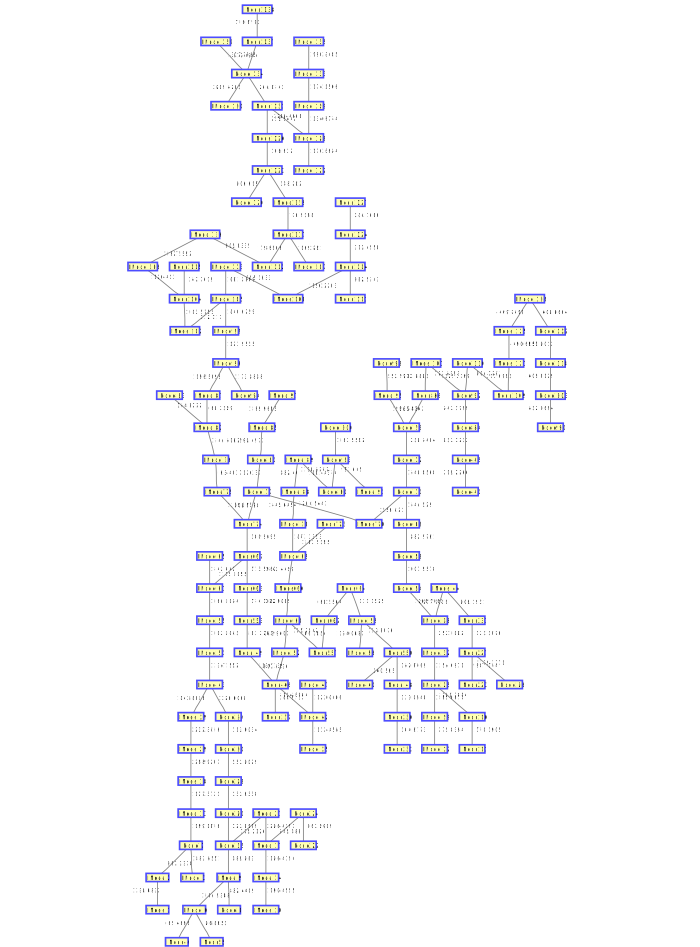
\includegraphics[width=16cm]{Biograph.eps}
	\caption{用最小生成树表示的总长度最短的网络连接方案} \label{shorttree}
\end{figure}

\restoregeometry

地图上的连接形式如图\ref{fig:最小生成树}。

\begin{figure}[htpb]
	\centering
	\includegraphics[width=0.8\linewidth]{shorttree.png}
	\caption{最小生成树}
	\label{fig:最小生成树}
\end{figure}

该连接方式的总长度为\SI{25342.188}{km}\cite{雷莉-412}。

\subsection{问题\chinese{subsection}:针对独立割点城市的战备节点配置模型}
\label{ssub:问题\chinese{subsection}:针对独立割点城市的战备节点配置模型}

\subsubsection{针对独立割点城市的战备节点数量确定}
\label{针对独立割点城市的战备节点数量确定}

由前述模型可知,当北京、武汉、上海三个互不连续的城市节点被摧毁时,战备节点的最佳数量为3个。

\subsubsection{针对独立割点城市的战备节点位置(地理坐标)确定}
\label{针对独立割点城市的战备节点位置(地理坐标)确定}

我们查阅资料得到北京、武汉、上海三个城市的实际面积,由此计算得到其安全距离及安全区域如表:

\begin{table}[htpb]
	\centering
	\caption{北京、武汉、上海三个城市的安全距离}
	\label{AB}
	\begin{tabu}to\linewidth{@{}X[c]X[c]X[c]X[c]@{}}
		\toprule
		城市 & 实际面积$S$        & 安全距离$R_{\text{safe}}$ & 安全范围$D_{\text{safe}}$                   \\
		\midrule
		北京 & \SI{16410.5}{km^2} & \SI{72.2746}{km}          & 以北京为圆心, \SI{72.2746}{km}为半径的圆外 \\
		武汉 & \SI{8494.41}{km^2} & \SI{51.9986}{km}          & 以武汉为圆心, \SI{51.9986}{km}为半径的圆外 \\
		上海 & \SI{6340.5}{km^2}  & \SI{44.9249}{km}          & 以上海为圆心, \SI{44.9249}{km}为半径的圆外 \\
		\bottomrule
	\end{tabu}
\end{table}

使用MATLAB\index{MATLAB}软件在前述约束条件下使目标函数最小,得到分别对应于北京、武汉、上海的战备节点的经纬度为:

\begin{table}[htpb]
	\centering
	\caption{对应于北京、武汉、上海的战备节点的经纬度}
	\label{AB}
	\begin{longtabu}to\linewidth{@{}X[c]X[c]X[c]@{}}
		\toprule
		战备节点 & 经度 & 纬度\\
		\midrule
		对应于北京的战备节点1 & \ang{115;47;13.46}&\ang{39;13;9.25}\\
		对应于武汉的战备节点2 & \ang{114;34;10.04}&\ang{31;10;32.04}\\
		对应于上海的战备节点3 & \ang{119;21;39.06}&\ang{31;32;30.07}\\
		\bottomrule
	\end{longtabu}
\end{table}

\begin{figure}[htpb]
	\centering
	\begin{subfigure}[htpb]{.31\linewidth}
		\centering
		\includegraphics[width=\linewidth]{211.png}
		\caption{战备节点\chinese{subfigure}}
		\label{fig:战备节点\chinese{subfigure}\arabic{subsection}}
	\end{subfigure}
	\quad
	\begin{subfigure}[htpb]{.31\linewidth}
		\centering
		\includegraphics[width=\linewidth]{221.png}
		\caption{战备节点\chinese{subfigure}}
		\label{fig:战备节点\chinese{subfigure}\arabic{subsection}}
	\end{subfigure}
	\quad
	\begin{subfigure}[htpb]{.31\linewidth}
		\centering
		\includegraphics[width=\linewidth]{231.png}
		\caption{战备节点\chinese{subfigure}}
		\label{fig:战备节点\chinese{subfigure}\arabic{subsection}}
	\end{subfigure}
	\caption{战备节点}
	\label{fig:战备节点\arabic{subsection}}
\end{figure}

\newpage

\subsection{问题\chinese{subsection}(1):针对割集城市的战备节点配置模型}%
\label{sub:\chinese{subsection}(1):针对割集城市的战备节点配置模型}

\subsubsection{针对割集城市的战备节点数量确定}
\label{针对割集城市的战备节点数量确定}

故宜昌、沙市、岳阳3个连续城市组成的割集对应一个战备节点,记为$Q_\mathrm{three}$,武汉、黄石、信阳、南昌、九江、安庆6个连续城市组成的割集对应另一个战备节点,记为$Q_\text{six}$。

\begin{figure}[htpb]
	\centering
	\begin{subfigure}[htpb]{.45\linewidth}
		\centering
		\includegraphics[width=\linewidth]{311.png}
		\caption{战备节点\chinese{subfigure}}
		\label{fig:战备节点\chinese{subfigure}\arabic{subsection}}
	\end{subfigure}
	\quad
	\begin{subfigure}[htpb]{.45\linewidth}
		\centering
		\includegraphics[width=\linewidth]{321.png}
		\caption{战备节点\chinese{subfigure}}
		\label{fig:战备节点\chinese{subfigure}\arabic{subsection}}
	\end{subfigure}
	\caption{战备节点}
	\label{fig:战备节点\arabic{subsection}}
\end{figure}

\subsubsection{针对割集城市的战备节点位置(地理坐标)确定}
\label{针对割集城市的战备节点位置(地理坐标)确定}

使用MATLAB\index{MATLAB}软件在前述约束条件下使目标函数最小,得到战备节点$Q_\text{three}$和$Q_\text{six}$的经纬度为:

\begin{table}[htpb]
	\centering
	\caption{对应于宜昌、沙市、岳阳、武汉、黄石、信阳、南昌、九江、安庆的战备节点的经纬度}
	\label{AB}
	\begin{longtabu}to\linewidth{@{}X[c]X[c]X[c]@{}}
		\toprule
		战备节点         & 经度 & 纬度 \\
		\midrule
		$Q_\text{three}$ &  \ang{111;43;07.04}    &  \ang{29;02;13.57}    \\
		$Q_\text{six}$   &  \ang{116;49;51.17}    &  \ang{31;33;32.67}    \\
		\bottomrule
	\end{longtabu}
\end{table}

\addtocounter{subsection}{-1}

\subsection{问题\chinese{subsection}(2):通信网络连通性能衡量模型}
\label{ssub:问题\chinese{subsection}(2):通信网络连通性能衡量模型}

我们使用MATLAB\index{MATLAB}软件,通过前述最大流算法\citesec{DspTian},求得问题一中通信网络中最小的最大流拓扑图\ref{fig:拓扑图}。

\begin{figure}[htpb]
	\centering
	\includegraphics[width=\linewidth]{4.png}
	\caption{拓扑图}
	\label{fig:拓扑图}
\end{figure}

我们计算得到该总长度最短的网络连接方案的连通度$\lambda=1$,畅通度为$\eta=100\%$,计算其网络连通能力因数为:
\begin{align}
	\xi=\eta \cdot \lambda=100\% \cdot 1=1
\end{align}

\subsection{问题\chinese{subsection}:通信网络综合优化模型}
\label{ssub:问题\chinese{subsection}:通信网络综合优化模型}

\subsubsection{求解兼顾抗攻击性和经济性的网络连接方案}
\label{求解兼顾抗攻击性和经济性的网络连接方案}
设问题一的连通图为$G$,依次找到三层关键节点,进行三层摧毁,增设线路进行修复连接,得到的\textbf{兼顾抗攻击性和经济性的最终网络连接方案}结果如图\ref{fig:兼顾抗攻击性和经济性的最终网络连接方案}(其中\textbf{红色连线}为增设线路):

\begin{figure}[htpb]
	\centering
	\includegraphics[width=0.8\linewidth]{43.png}
	\caption{兼顾抗攻击性和经济性的最终网络连接方案}
	\label{fig:兼顾抗攻击性和经济性的最终网络连接方案}
\end{figure}

我们用数字标号表示每层的关键节点。其中,

一层关键节点:$K=1$

二层关键节点:$K_1=2,K_2=3,K_3=4,K_4=5$

三层关键节点:$K_{11}=7,K_{12}=13,K_{21}=6,K_{22}=8,K_{23}=9,K_{24}=10,K_{31}=11,K_{32}=12,K_{33}=14$

关键节点共计14个,占总节点数139的比例为:

\begin{align}
	\sigma=\frac{14}{139}\cdot 100\%=10.07\%>10\%
\end{align}

鉴于问题四最后要求模拟$10\%$的节点被摧毁时的网络连通性能\cite{岳超-410},因此我们的优化方案使得摧毁$10\%$的节点后存在所有链路全部正常通信的可能性,验证了模型的合理性。

同时,我们考虑到题目中所要求的“务必确保重要城市在通信网络中的连通性能”,我们根据城市在实际生活中在交通、经济、政治等方面的重要程度,在139个城市中分别\textbf{在中国的“东、西、南、北、中”各选择一个重要城市},分别为上海、乌鲁木齐、广州、北京、武汉。

借鉴现代交换技术中核心设备交换机的冗余度策略,我们对上述五个“重要城市”进行“冗余保护策略”,即增设两条重要城市与邻近未连接城市的连线(在图\ref{fine}中用\textbf{黄色连线}表示),以增加重要城市的通信线路冗余度,从而当原本与重要城市直接相连的城市被摧毁时,重要城市仍能通过冗余线路进行正常通信,确保了重要城市的连通性能。在这种情况下,整个网络的联通性能也得到提升,进一步优化了连接方案。

\subsubsection{模拟摧毁后的网络连通性能测算}
\label{模拟摧毁后的网络连通性能测算}

我们使用MATLAB产生1-139中的14(占139的10\%)数,对应14个城市,分别是:柳州,三明,吐鲁番,武汉,黄石,天水,格尔木,宝鸡,太原,银川,锦州,阿克苏,呼和浩特,汉中。

将这14个城市节点及与其直接相连的连线摧毁,即将它们从通信链路上删除,得到如下的摧毁后的通信网络:

\begin{figure}[htpb]
	\centering
	\includegraphics[width=0.8\linewidth]{44.png}
	\caption{摧毁后的通信网络}
	\label{fig:摧毁后的通信网络}
\end{figure}

我们使用MATLAB软件,通过前述最大流算法,求得该摧毁后的通信网络的连通度$\lambda=1$。计算其畅通度$\eta=72.6\%$,计算其网络连通能力因数为:
\begin{align}
	\xi=\eta \cdot \lambda=72.6\% \cdot 1=0.726
\end{align}

可见,摧毁10\%的节点使得网络连通能力下降27.4\%,考虑到经济性的尽可能提升,这一结果已可以接受。

\section{模型的评价}%
\label{sec:模型的评价}

\subsection{优点}%
\label{sub:优点}

\begin{enumerate}
	\item 在文章起始处就明确地将通讯网络的设计与抗毁性研究问题转换成了数学几何问题,并归属于图论问题,将题目中的城市等要素类比为图论中的节点等要素。
	\item 运用最小生成树算法求解总长度最短的网络连接方案具有很强的普适性,且可以作为后续问题中对网络改进的基础。
	\item 从对独立割点和割点集的摧毁两种情况考虑战备节点的设置问题,具有普适性。
	\item 构建了合理的通信网络连通性能衡量模型,将连通度和畅通度结合,不仅能判断连通图的连通性能,还可以判断非连通图的连通性能。
	\item 使用重要节点强制摧毁算法,采用分级条件法处理经济型与抗攻击性的权衡,层层递进,且可以通过增加层数来进一步提高连通性能,具有很强的移植性。
\end{enumerate}

\subsection{缺点}%
\label{sub:缺点}

\begin{enumerate}
	\item 在考虑连通度的计算时,仅考虑了边连通度,没有分析点连通度对连通性能的影响;
	\item 畅通度的定义合理性不强,简单地使用包含最大点数的子图的点数与总网络点数的比值,但实际上包含较少点数的子图内部仍然可以正常通信,我们没有将其以某种合适的方式考虑进整个网络连通性能的评价体系当中。
	\item 在强制摧毁算法中我们进行了三层摧毁,虽然保证了经济性的优良,但最终摧毁10\%节点后的网络连通性能并不太高,我们没有找到判断经济性达标的阈值,没有找到最终摧毁10\%节点后的网络连通性能与摧毁算法层数之间的确定关系。
	\item 构建了合理的通信网络连通性能衡量模型,将连通度和畅通度结合,不仅能判断连通图的连通性能,还可以判断非连通图的连通性能。
\end{enumerate}

\newpage

% Fakesection 参考文献

\bibliography{src/main}
\bibliographysec{src/B028819084}

\newpage

% Fakesection 附录

\ifNoAppendix
	\else

		\renewcommand{\thesection}{\Alph{section}~}

		\appendix

		\section{代码}%
		\label{sec:代码}

		\langCVfile[Matlab][code:1][Matlab]{Biograph.m}{src/Biograph.m}

		\langCVfile[Matlab][code:2][Matlab]{code3.m}{src/code3.m}

		\langCVfile[Matlab][code:3][Matlab]{code4.m}{src/code4.m}

		\langCVfile[Matlab][code:4][Matlab]{connectivity.m}{src/connectivity.m}

		\langCVfile[Matlab][code:5][Matlab]{code.m}{src/code.m}

		\section{运行结果}%
		\label{sec:运行结果}

		%%MatLab命令行
		\newcommand{\MatlabLogo}{%
			\begin{tikzpicture}[x=2.4ex,y=2.4ex,line width=0ex,scale=1]
				\node[draw,fill=white,text=white] at (0, 0) (a) {
						\includegraphics[width=2.4ex]{matlabLogo.ai}
					};
			\end{tikzpicture}
		}
		\tcbset{%
			skin=enhanced,%
			matlab/.style={%
				skin=bicolor,%
				boxrule=0.1mm,%
				%toptitle=1ex,
				sharp corners,
				breakable,%
				colbacktitle=WinGray,%
				colframe=WinGray,%
				coltitle=black,%
				fonttitle=\sffamily,%\bfseries,
				fontupper=\small\sffamily,
				fontlower=\small\sffamily,
				frame style={%
					draw=WinBlue,%
					left color=WinBlue,%
					right color=WinBlue%
				},%
				overlay unbroken = {%
					\node[inner sep=0pt,anchor=north west,yshift=-3pt,xshift=1.2pt,text=black]
					at (frame.north west){\MatlabLogo};% \fbox{\faTerminal}
					\node[inner sep=0pt,anchor=north east,yshift=-3pt,xshift=-8pt,text=black] at (frame.north
					east){\rule{0.8em}{0.6pt}\quad$\square$\quad{\Large$\times$}};
				},%
				overlay first = {%
					\node[inner sep=0pt,anchor=north west,yshift=-3pt,xshift=1.0pt,text=black]
					at (frame.north west){\MatlabLogo};%\small ~\faWindows
					\node[inner sep=0pt,anchor=north east,yshift=-3pt,xshift=-8pt,text=black] at (frame.north
					east){\rule{0.8em}{0.6pt}\quad$\square$\quad{\Large$\times$}};
				}%
			},
			matlablight/.style={
				matlab,%
				colback=white,%
				colupper=black,%
				%coltext=black%
			},
			matlabdark/.style={
				matlab,%
				colback=black,%
				colupper=white,%
				%coltext=white%
			}
		}
		\DeclareTCBListing{matlabdarkc}{ m m }{%
			listing engine=minted,%
			minted style=trac,%
			minted options={%
				autogobble,%
				breaklines,%
				fontsize=\wuhao,%
				baselinestretch=0.6,%
				breaksymbolleft={},%
				numbersep=3mm%
			},%
			listing and comment,%
			colbacklower=tcbcol@back!5!yellow!10!white,%
			collower=linux,%
			matlabdark,%
			title={#2},%
			comment={\small\sffamily#1},%
			minted language=bat%
		}
		\DeclareTCBListing{matlablightc}{ m m }{%
			listing engine=minted,%
			minted style=trac,%
			minted options={%
				autogobble,%
				breaklines,%
				fontsize=\wuhao,%
				baselinestretch=0.6,%
				breaksymbolleft={},%
				numbersep=3mm%
			},%
			listing and comment,%
			colbacklower=tcbcol@back!5!yellow!10!white,%
			collower=linux,%
			matlablight,%
			title={#2},%
			comment={\small\sffamily#1},%
			minted language=bat%
		}
		\DeclareTCBListing{matlabdark}{ m }{%
			listing engine=minted,%
			minted style=trac,%
			minted options={%
				autogobble,%
				breaklines,%
				fontsize=\wuhao,%
				baselinestretch=0.6,%
				breaksymbolleft={},%
				numbersep=3mm%
			},%
			listing only,%
			matlabdark,%
			title={#1},%
			minted language=bat%
		}
		\DeclareTCBListing{matlablight}{ m }{%
			listing engine=minted,%
			minted style=trac,%
			minted options={%
				autogobble,%
				breaklines,%
				fontsize=\wuhao,%
				baselinestretch=0.6,%
				breaksymbolleft={},%
				numbersep=3mm%
			},%
			listing only,%
			matlablight,%
			title={#1},%
			minted language=bat%
		}
		\newtcbinputlisting{\matlabdarkcfile}[3]{%
			listing engine=minted,%
			minted style=trac,%
			minted options={%
				autogobble,%
				breaklines,%
				fontsize=\wuhao,%
				baselinestretch=0.6,%
				breaksymbolleft={},%
				numbersep=3mm%
			},%
			listing and comment,%
			colbacklower=tcbcol@back!5!yellow!10!white,%
			collower=linux,%
			matlabdark,%
			listing file={#3},
			title={#2},%
			comment={\small\sffamily#1},%
			minted language=bat%
		}% end matlabdarkcfile
		% 将文件做为窗口内容的Windows终端窗口样式命令
		% 第1个参数是窗口底端提示信息
		% 第2个参数是窗口标题
		% 第3个参数是包含窗口内容的文件全路径名称(可以是相对路径)
		\newtcbinputlisting{\matlablightcfile}[3]{%
			listing engine=minted,%
			minted style=trac,%
			minted options={%
				autogobble,%
				breaklines,%
				fontsize=\wuhao,%
				baselinestretch=0.6,%
				breaksymbolleft={},%
				numbersep=3mm%
			},%
			listing and comment,%
			colbacklower=tcbcol@back!5!yellow!10!white,%
			collower=linux,%
			matlablight,%
			listing file={#3},
			title={#2},%
			comment={\small\sffamily#1},%
			minted language=bat%
		}% end matlablightcfile
		% 将文件做为窗口内容的Windows终端窗口样式命令
		% 第1个参数是窗口标题
		% 第2个参数是包含窗口内容的文件全路径名称(可以是相对路径)
		\newtcbinputlisting{\matlabdarkfile}[2]{%
			listing engine=minted,%
			minted style=trac,%
			minted options={%
				autogobble,%
				breaklines,%
				fontsize=\wuhao,%
				baselinestretch=0.6,%
				breaksymbolleft={},%
				numbersep=3mm%
			},%
			listing only,%
			matlabdark,%
			listing file={#2},
			title={#1},%
			minted language=bat%
		}% end matlabdarkfile
		% 将文件做为窗口内容的Windows终端窗口样式命令
		% 第1个参数是窗口标题
		% 第2个参数是包含窗口内容的文件全路径名称(可以是相对路径)
		\newtcbinputlisting{\matlablightfile}[2]{%
			listing engine=minted,%
			minted style=trac,%
			minted options={%
				autogobble,%
				breaklines,%
				fontsize=\wuhao,%
				baselinestretch=0.6,%
				breaksymbolleft={},%
				numbersep=3mm%
			},%
			listing only,%
			matlablight,%
			listing file={#2},
			title={#1},%
			minted language=bat%
		}% end matlablightfile

		\matlablightfile{MATLAB Command Window}{src/Biograph.txt}

		% Fakesection 索引

		\printindex

	\fi

	\end{document}

